\documentclass{standalone}
\usepackage{tikz}
\usepackage{verbatim}
\usetikzlibrary{positioning}
\begin{document}
\pagestyle{empty}
  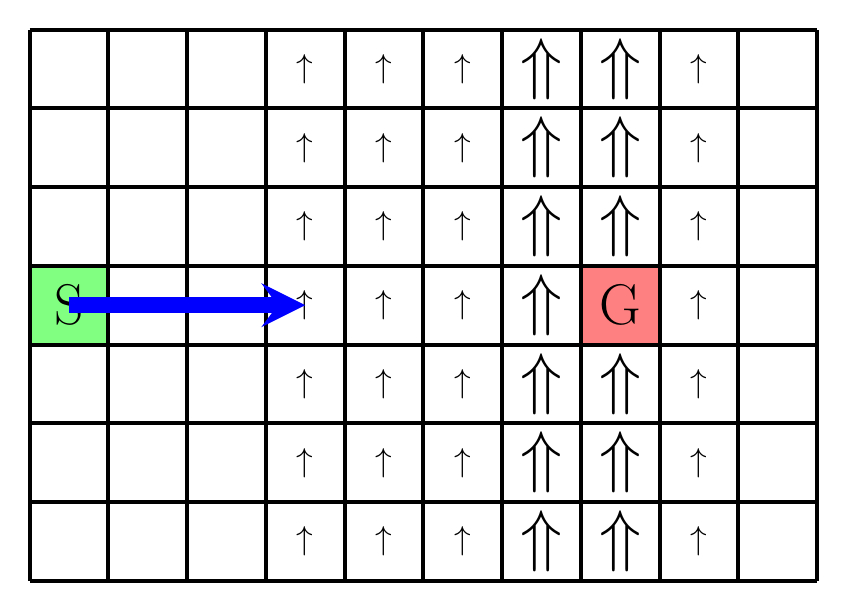
\begin{tikzpicture}

    \fill[green!50] (0, 3) rectangle (1,4);
    \node at (0.5, 3.5) {\huge S};
    \foreach \y in {0,1,2,3,4,5,6} {
      \node at (3.5, \y + 0.5) {\large $\uparrow$};
      \node at (4.5, \y + 0.5) {\large $\uparrow$};
      \node at (5.5, \y + 0.5) {\large $\uparrow$};
      \node at (6.5, \y + 0.5) {\Huge $\Uparrow$};
      \node at (7.5, \y + 0.5) {\Huge $\Uparrow$};
      \node at (8.5, \y + 0.5) {\large $\uparrow$};
	 }
	 \fill[red!50] (7, 3) rectangle (8,4);
    \node at (7.5, 3.5) {\huge G};

    \draw[step=1.0,black, line width=0.5 mm] (0,0) grid (10, 7);
    
    \draw[-stealth, line width=2 mm, blue] (0.5, 3.5) -- (3.5,3.5);
  \end{tikzpicture}
\end{document}